\ifthenelse{\boolean{abridgeConics}}{}{%
\printconcepts

\exercise{What is the difference between degenerate and nondegenerate conics?}{When defining the conics as the intersections of a plane and a double napped cone, degenerate conics are created when the plane intersects the tips of the cones (usually taken as the origin). Nondegenerate conics are formed when this plane does not contain the origin.}

\exercise{Use your own words to explain what the eccentricity of an ellipse measures.}{Answers will vary.}

\exercise{What has the largest eccentricity: an ellipse or a hyperbola?}{Hyperbola}

\exercise{Explain why the following is true: ``If the coefficient of the $x^2$ term in the equation of an ellipse in standard form is smaller than the coefficient of the $y^2$ term, then the ellipse has a horizontal major axis.''}{With the equation $\frac{(x-h)^2}{a^2}+\frac{(y-k)^2}{b^2}=1$, the ellipse has a horizontal major axis if $a>b$. But the coefficient of the $x^2$ term is $1/a^2$ (not $a^2$), so if $1/a^2<1/b^2$, then $a>b$ and the major axis is horizontal.}

\exercise{Explain how one can quickly look at the equation of a hyperbola in standard form and determine whether the transverse axis is horizontal or vertical.}{With a horizontal transverse axis, the $x^2$ term has a positive coefficient; with a vertical transverse axis, the $y^2$ term has a positive coefficient.}
}

\printproblems

\input{exercises/09_01_exset_01}

\ifthenelse{\boolean{abridgeConics}}{}{\begin{exerciseset}{In Exercises}{, the equation of a parabola and a point on its graph are given. Find the focus and directrix of the parabola, and verify that the given point is equidistant from the focus and directrix.}

\exercise{$y=\frac14x^2$, $P=(2,1)$}{focus: $(0,1)$; directrix: $y=-1$. The point $P$ is 2 units from each.}

\exercise{$x=\frac18(y-2)^2+3$, $P=(11,10)$}{focus: $(5,2)$; directrix: $x=1$. The point $P$ is 10 units from each.}

\end{exerciseset}
}

\exerciseset{In Exercises}{, sketch the ellipse defined by the given equation. Label the center, foci and vertices.}{

\exercise{$\dfrac{(x-1)^2}{3}+\dfrac{(y-2)^2}{5}=1$}{\mbox{}\\[-\baselineskip]
\begin{tikzpicture}[scale=.75]
\begin{axis}[width=1.16\marginparwidth,tick label style={font=\scriptsize},
axis y line=middle,axis x line=middle,name=myplot,axis equal,
ymin=-1,ymax=5,xmin=-1.1,xmax=3.2]
\addplot [thick, smooth,domain=0:360,samples=60] ({1.73*cos(x)+1},{2.24*sin(x)+2});
\filldraw (axis cs: 1,2) circle (1.5pt)
                                        (axis cs: 1,4.24) circle (1.5pt)
                                        (axis cs: 1,-.24) circle (1.5pt);
\ifthenelse{\boolean{abridgeConics}}{}{
\filldraw (axis cs: 1,3.4) circle (1.5pt) (axis cs: 1,.6) circle (1.5pt);
}
\end{axis}
\node [right] at (myplot.right of origin) {\scriptsize $x$};
\node [above] at (myplot.above origin) {\scriptsize $y$};
\end{tikzpicture}
}

\exercise{$\dfrac{1}{25}x^2+\dfrac{1}{9}(y+3)^2=1$}{\mbox{}\\[-\baselineskip]
\begin{tikzpicture}[scale=.75]
\begin{axis}[width=1.16\marginparwidth,tick label style={font=\scriptsize},
axis y line=middle,axis x line=middle,name=myplot,axis equal,
ymin=-6.5,ymax=1.5,xmin=-5.5,xmax=5.5]
\addplot [thick, smooth,domain=0:360,samples=60] ({5*cos(x)},{3*sin(x)-3});
\filldraw (axis cs: 0,-3) circle (1.5pt)
                                        (axis cs: -5,-3) circle (1.5pt)
                                        (axis cs: 5,-3) circle (1.5pt);
\ifthenelse{\boolean{abridgeConics}}{}{
\filldraw(axis cs: -4,-3) circle (1.5pt) (axis cs: 4,-3) circle (1.5pt);
}
\end{axis}
\node [right] at (myplot.right of origin) {\scriptsize $x$};
\node [above] at (myplot.above origin) {\scriptsize $y$};
\end{tikzpicture}
}

}


\exerciseset{In Exercises}{, find the equation of the ellipse shown in the graph.% Give the location of the foci and the eccentricity of the ellipse.
}{

\exercise{\begin{minipage}{\linewidth}\centering\myincludegraphics[scale=.8]{figures/fig09_01_ex_20}\end{minipage}}{$\frac{(x+1)^2}{9}+\frac{(y-2)^2}{4}=1$; foci at $(-1\pm\sqrt{5},2)$; $e=\sqrt{5}/3$}

\exercise{\begin{minipage}{\linewidth}\centering\myincludegraphics[scale=.8]{figures/fig09_01_ex_21}\end{minipage}}{$\frac{(x-1)^2}{1/4}+\frac{y^2}{9}=1$; foci at $(1,\pm \sqrt{8.75})$; $e=\sqrt{8.75}/3\approx 0.99$}

}


\ifthenelse{\boolean{abridgeConics}}{}{\input{exercises/09_01_exset_04}}

\input{exercises/09_01_exset_06}

\ifthenelse{\boolean{abridgeConics}}{}{%
\exercise{Consider the ellipse given by $\ds \frac{(x-1)^2}{4}+\frac{(y-3)^2}{12}=1$.
\begin{enumerate}
\item		Verify that the foci are located at $(1,3\pm 2\sqrt{2})$.
\item		The points $P_1 = (2,6)$ and $P_2 = (1+\sqrt{2},3+\sqrt{6}) \approx (2.414,5.449)$ lie on the ellipse. Verify that the sum of distances from each point to the foci is the same.
\end{enumerate}
}{\begin{enumerate}
\item		$c=\sqrt{12-4} = 2\sqrt{2}$.
\item		The sum of distances for each point is $2\sqrt{12}\approx 6.9282$. 
\end{enumerate}}
}

\exerciseset{In Exercises}{, find the equation of the hyperbola shown in the graph.
}{

\exercise{\noindent\begin{minipage}{\linewidth}\centering \myincludegraphics[scale=.8]{figures/fig09_01_ex_27}\end{minipage}
}{$x^2-\frac{y^2}{3}=1$
}

\exercise{\noindent\begin{minipage}{\linewidth}\centering \myincludegraphics[scale=.8]{figures/fig09_01_ex_28}\end{minipage}
}{$y^2-\frac{x^2}{24}=1$
}

\exercise{\noindent\begin{minipage}{\linewidth}\centering \myincludegraphics[scale=.8]{figures/fig09_01_ex_29}\end{minipage}
}{$\frac{(y-3)^2}{4}-\frac{(x-1)^2}{9}=1$
}

\exercise{\noindent\begin{minipage}{\linewidth}\centering \myincludegraphics[scale=.8]{figures/fig09_01_ex_30}\end{minipage}
}{$\frac{(x-1)^2}{9}-\frac{(y-3)^2}{4}=1$
}
}

\exerciseset{In Exercises}{, sketch the hyperbola defined by the given equation. Label the center.% and foci.
}{

\exercise{$\ds \frac{(x-1)^2}{16}-\frac{(y+2)^2}{9}=1$}{
\begin{tikzpicture}
\begin{axis}[width=\marginparwidth+25pt,tick label style={font=\scriptsize},
axis y line=middle,axis x line=middle,name=myplot,
minor x tick num=4,minor y tick num=1,ymin=-6.5,ymax=2.5,xmin=-6.5,xmax=7.5]

\addplot [thick, smooth,domain=-70:70,samples=30] ({4*sec(x)+1},{3*tan(x)-2});
\addplot [thick, smooth,domain=-70:70,samples=30] ({-4*sec(x)+1},{3*tan(x)-2});

\filldraw (axis cs: 6,-2) circle (1.5pt)
                                        (axis cs: -4,-2) circle (1.5pt)
                                        (axis cs: 1,-2) circle (1.5pt)
                                        (axis cs: 5,-2) circle (1.5pt)
                                        (axis cs: -3,-2) circle (1.5pt);
\end{axis}

\node [right] at (myplot.right of origin) {\scriptsize $x$};
\node [above] at (myplot.above origin) {\scriptsize $y$};
\end{tikzpicture}
}

\exercise{$\ds (y-4)^2-\frac{(x+1)^2}{25}=1$}{
\begin{tikzpicture}
\begin{axis}[width=\marginparwidth+25pt,tick label style={font=\scriptsize},
axis y line=middle,axis x line=middle,name=myplot,
minor x tick num=4,minor y tick num=4,ymin=-2.5,ymax=10.5,xmin=-10.5,xmax=9.5]

\addplot [thick, smooth,domain=-70:70,samples=30] ({5*tan(x)-1},{sec(x)+4});
\addplot [thick, smooth,domain=-70:70,samples=30] ({5*tan(x)-1},{-sec(x)+4});

\filldraw (axis cs: -1,9.1) circle (1.5pt)
                                        (axis cs: -1,-1.1) circle (1.5pt)
                                        (axis cs: -1,4) circle (1.5pt)
                                        (axis cs: -1,5) circle (1.5pt)
                                        (axis cs: -1,3) circle (1.5pt);
\end{axis}

\node [right] at (myplot.right of origin) {\scriptsize $x$};
\node [above] at (myplot.above origin) {\scriptsize $y$};
\end{tikzpicture}
}

}


\ifthenelse{\boolean{abridgeConics}}{}{\exerciseset{In Exercises}{, find the equation of the hyperbola defined by the given information. Sketch the hyperbola.
}{

\exercise{Foci: $(\pm 3,0)$; vertices: $(\pm 2, 0)$
}{$\frac{x^2}{4}-\frac{y^2}{5}=1$
}

\exercise{Foci: $(0,\pm 3)$; vertices: $(0,\pm 2)$
}{$\frac{y^2}{4}-\frac{x^2}{5}=1$
}

\exercise{Foci: $(-2,3)$ and $(8,3)$; vertices: $(-1,3)$ and $(7,3)$
}{$\frac{(x-3)^2}{16}-\frac{(y-3)^2}{9}=1$
}

\exercise{Foci: $(3,-2)$ and $(3,8)$; vertices: $(3,0)$ and $(3,6)$
}{$\frac{(y-3)^2}{9}-\frac{(x-3)^2}{16}=1$
}
}}

\exerciseset{In Exercises}{, write the equation of the hyperbola in standard form.
}{

\exercise{$3x^2-4y^2=12$
}{$\frac{x^2}{4}-\frac{y^2}{3}=1$
}

\exercise{$3x^2-y^2+2y=10$
}{$\frac{x^2}{3}-\frac{(y-1)^2}{9}=1$
}

\exercise{$x^2-10y^2+40y=30$
}{$(y-2)^2-\frac{x^2}{10}=1$
}

\exercise{$(4y-x)(4y+x)=4$
}{$4y^2-\frac{x^2}{4}=1$
}
}

\ifthenelse{\boolean{abridgeConics}}{}{%
\exercise{Johannes Kepler discovered that the planets of our solar system have elliptical orbits with the Sun at one focus. The Earth's elliptical orbit is used as a standard unit of distance; the distance from the center of Earth's elliptical orbit to one vertex is 1 Astronomical Unit, or A.U. 

The following table gives information about the orbits of three planets.

\begin{center}
\begin{tabular}{ccc}
Planet & \parbox{80pt}{\centering Distance from center to vertex (A.U.)} & eccentricity \\ \midrule
Mercury & 0.387 & 0.2056 \\
Earth & 1\phantom{.000} & 0.0167 \\
Mars & 1.524 & 0.0934 
\end{tabular}
\end{center}

\begin{enumerate}
\item		In an ellipse, knowing $c^2=a^2-b^2$ and $e=c/a$ allows us to find $b$ in terms of $a$ and $e$. Show $b=a\sqrt{1-e^2}$. 
\item		For each planet, find equations of their elliptical orbit of the form $\ds\frac{x^2}{a^2}+\frac{y^2}{b^2}=1$. (This places the center at $(0,0)$, but the Sun is in a different location for each planet.)
\item		Shift the equations so that the Sun lies at the origin. Plot the three elliptical orbits.
\end{enumerate}}{\begin{enumerate}
\item		Solve for $c$ in $e=c/a$: $c=ae$. Thus $a^2e^2=a^2-b^2$, and $b^2=a^2-a^2e^2$. The result follows.
\item		Mercury: $x^2/(0.387)^2 + y^2/(0.3787)^2=1$	\\
				Earth:	$x^2+y^2/(0.99986)^2 = 1$\\
				Mars:   $x^2/(1.524)^2+y^2/(1.517)^2=1$
\item		Mercury: $(x-0.08)^2/(0.387)^2 + y^2/(0.3787)^2=1$	\\
				Earth:  $(x-0.0167)^2+y^2/(0.99986)^2 = 1$\\
				Mars:   $(x-0.1423)^2/(1.524)^2+y^2/(1.517)^2=1$
\end{enumerate}}

\exercise{A loud sound is recorded at three stations that lie on a line as shown in the figure below. Station $A$ recorded the sound 1 second after Station $B$, and Station $C$ recorded the sound 3 seconds after $B$. Using the speed of sound as 340m/s, determine the location of the sound's origination.

\hfill 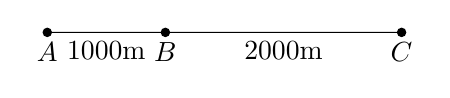
\begin{tikzpicture}
\draw [fill=black] (0,0) circle (1.5pt) node [below] {$A$}  -- node [pos=.5,below] {1000m} (1.5,0) circle (1.5pt) node [below] {$B$} -- node [pos=.5,below] {2000m} (4.5,0) circle (1.5pt) node [below] {$C$};
\end{tikzpicture} \hfill \null}{The sound originated from a point approximately 31m to the left of $B$ and 1340m above it.}
}
